\documentclass[12pt,a4paper,fontset=none]{ctexart}

\usepackage[margin=1in]{geometry}
\usepackage{graphicx}
\usepackage{amsmath}
\usepackage{array}
\usepackage{hyperref}

\hypersetup{
    colorlinks=true,
    linkcolor=black,
    urlcolor=blue,
    citecolor=black
}

\graphicspath{
    {../outputs/search_32_best/plots/}
    {../outputs/final_32_test/plots/}
}

\setCJKmainfont{Noto Serif CJK SC}
\setCJKsansfont{Noto Sans CJK SC}
\setCJKmonofont{Noto Sans CJK SC}

\newcommand{\StudentName}{\underline{\makebox[4cm][c]{姚宗骏}}}
\newcommand{\StudentID}{\underline{\makebox[4cm][c]{25110980027}}}
\newcommand{\RepoURL}{\url{https://github.com/zj-yao/EuroSAT}}
\newcommand{\WeightURL}{\texttt{[提交前填写模型权重下载链接]}}

\title{从零开始构建三层神经网络分类器\\EuroSAT 地表覆盖图像分类实验报告}
\author{姓名：\StudentName \quad 学号：\StudentID}
\date{\today}

\begin{document}

\maketitle

\begin{abstract}
本报告基于 EuroSAT RGB 数据集，使用纯 \texttt{NumPy} 从零实现自动微分、三层多层感知机
（MLP）、随机梯度下降（SGD）、学习率衰减、交叉熵损失与 $L_2$ 正则化，并完成训练、
超参数搜索、测试评估、权重可视化与错例分析。实验中采用分层划分构造训练集、验证集和
测试集，图像统一缩放到 $32 \times 32$，输入维度为 3072。最终在测试集上获得
\textbf{62.62\%} 的分类准确率，相比基线模型的 \textbf{61.38\%} 提升了约
\textbf{1.23} 个百分点。结果表明，在不使用卷积结构的前提下，三层 MLP 已经可以学习到
一定的颜色与粗纹理判别模式，但在 Highway、HerbaceousVegetation、PermanentCrop 等
类别上仍然存在较明显的混淆。
\end{abstract}

\section{任务概述}

本次作业的目标是在不依赖 PyTorch、TensorFlow、JAX 等自动微分框架的前提下，
从零实现一个三层神经网络分类器，在 EuroSAT 遥感图像数据集上完成 10 类地表覆盖分类。
根据作业要求，实验系统至少需要包含以下五个模块：

\begin{enumerate}
    \item 数据加载与预处理；
    \item 模型定义；
    \item 训练循环；
    \item 测试评估；
    \item 超参数搜索。
\end{enumerate}

本项目的代码实现位于 \texttt{src/} 目录下，核心模块包括
\texttt{autograd.py}、\texttt{dataset.py}、\texttt{model.py}、
\texttt{train.py}、\texttt{test.py} 与 \texttt{search.py}。

\section{数据集与预处理}

\subsection{数据集}

EuroSAT RGB 数据集共包含 10 个类别，类别顺序按文件夹名称排序为：
\texttt{AnnualCrop}、\texttt{Forest}、\texttt{HerbaceousVegetation}、
\texttt{Highway}、\texttt{Industrial}、\texttt{Pasture}、
\texttt{PermanentCrop}、\texttt{Residential}、\texttt{River}、
\texttt{SeaLake}。

实验中采用分层随机划分，比例为 70\% / 15\% / 15\%。
实际划分结果为：

\begin{itemize}
    \item 训练集：18900 张；
    \item 验证集：4050 张；
    \item 测试集：4050 张。
\end{itemize}

\subsection{预处理流程}

为了降低纯 MLP 在 CPU 上的训练开销，实验将原始 RGB 图像统一缩放到
$32 \times 32$。之后对训练集像素计算通道均值与标准差，对全部样本进行标准化，
并将图像展平为一维向量作为 MLP 输入，因此每个样本的输入维度为：

\begin{equation}
    d = 32 \times 32 \times 3 = 3072.
\end{equation}

整个预处理流程如下：

\begin{enumerate}
    \item 读取图像并转换为 RGB；
    \item 缩放到 $32 \times 32$；
    \item 将像素值归一化到 $[0,1]$；
    \item 使用训练集统计量做逐通道标准化；
    \item 将图像展平成长度为 3072 的向量。
\end{enumerate}

\section{模型与方法}

\subsection{自动微分实现}

项目自行实现了一个轻量级 \texttt{Tensor} 类，支持计算图构建、拓扑排序和反向传播。
目前实现了加法、减法、乘法、除法、矩阵乘法、求和以及 ReLU、Tanh、Sigmoid 等操作，
并在反向传播阶段自动累积梯度。这使得训练过程无需依赖现成深度学习框架的自动微分机制。

\subsection{三层 MLP 结构}

本实验使用三层全连接网络：

\begin{equation}
    h_1 = \phi(W_1 x + b_1), \quad
    h_2 = \phi(W_2 h_1 + b_2), \quad
    z = W_3 h_2 + b_3,
\end{equation}

其中 $\phi(\cdot)$ 为激活函数，$z$ 为类别 logits。
模型支持在 ReLU、Tanh、Sigmoid 之间切换；在最终最佳配置中，采用的是 ReLU。

\subsection{损失函数与优化}

训练阶段采用 Softmax 交叉熵损失：

\begin{equation}
    \mathcal{L}_{ce} =
    - \frac{1}{N} \sum_{i=1}^{N}
    \log \frac{e^{z_{i,y_i}}}{\sum_{c} e^{z_{i,c}}}.
\end{equation}

参数更新使用 SGD，并在梯度中显式加入 $L_2$ 正则项（Weight Decay）：

\begin{equation}
    \theta \leftarrow \theta - \eta \left( \nabla_{\theta}\mathcal{L}_{ce} + \lambda \theta \right).
\end{equation}

学习率衰减采用 Step LR 调度器：每经过 5 个 epoch，将学习率乘以 0.5。
此外，程序会在验证集准确率提升时自动保存当前最优模型权重。

\section{实验设置}

\subsection{基线模型}

基线模型的配置如下：

\begin{itemize}
    \item 图像尺寸：$32 \times 32$；
    \item 隐藏层维度：\texttt{[128, 64]}；
    \item 激活函数：ReLU；
    \item 学习率：0.01；
    \item Weight Decay：$10^{-4}$；
    \item 训练轮数：30。
\end{itemize}

\subsection{超参数搜索}

为了得到更优配置，实验进行了 8 组随机搜索，候选空间如下：

\begin{itemize}
    \item 学习率：\{0.1, 0.03, 0.01, 0.003\}；
    \item 隐藏层维度：\{[128,64], [256,128]\}；
    \item Weight Decay：\{0, $10^{-4}$, $10^{-3}$\}；
    \item 激活函数：\{\texttt{relu}, \texttt{tanh}\}。
\end{itemize}

每组搜索训练 20 个 epoch，并以验证集最佳准确率作为模型选择标准。

\begin{table}[htbp]
\centering
\small
\begin{tabular}{|c|c|c|c|c|c|}
\hline
Trial & LR & Hidden Dims & Weight Decay & Activation & Best Val Acc (\%) \\
\hline
01 & 0.003 & [128, 64] & 0 & tanh & 52.40 \\
02 & 0.01 & [256, 128] & 0 & relu & 61.56 \\
03 & 0.003 & [256, 128] & $10^{-4}$ & tanh & 54.15 \\
04 & 0.01 & [256, 128] & $10^{-3}$ & relu & 61.70 \\
05 & 0.1 & [128, 64] & $10^{-3}$ & tanh & 60.74 \\
06 & 0.003 & [256, 128] & $10^{-3}$ & tanh & 54.10 \\
07 & 0.003 & [256, 128] & $10^{-4}$ & relu & 56.49 \\
08 & 0.01 & [128, 64] & 0 & relu & 59.85 \\
\hline
\end{tabular}
\caption{8 组随机搜索结果}
\label{tab:search_results}
\end{table}

最终选出的最佳配置为：
\texttt{lr=0.01}，\texttt{hidden\_dims=[256,128]}，
\texttt{weight\_decay=0.001}，\texttt{activation=relu}。

\section{实验结果}

\subsection{基线模型与最终模型对比}

\begin{table}[htbp]
\centering
\begin{tabular}{|c|c|c|c|c|c|}
\hline
模型 & Hidden Dims & Weight Decay & Epochs & Best Val Acc (\%) & Test Acc (\%) \\
\hline
Baseline\_32 & [128, 64] & $10^{-4}$ & 30 & 60.10 & 61.38 \\
Search\_32\_Best & [256, 128] & $10^{-3}$ & 20 & 61.70 & 62.62 \\
\hline
\end{tabular}
\caption{基线模型与最终模型对比}
\label{tab:baseline_final}
\end{table}

可以看到，经过超参数搜索后，最终模型在测试集上的准确率从 61.38\% 提升到 62.62\%，
提升约 1.23 个百分点；测试损失也从 1.086 降低到 1.065。说明增大隐藏层宽度、
适当加强正则化，对该任务是有益的。

\subsection{训练过程曲线}

图~\ref{fig:training_curves} 展示了最终模型的训练集损失、验证集损失和验证集准确率曲线。
可以看到：

\begin{itemize}
    \item 前 5 个 epoch 收敛最快，损失下降明显；
    \item 验证集准确率在第 15 个 epoch 左右达到峰值，之后进入平台期；
    \item 训练损失与验证损失之间存在一定间隔，但没有出现剧烈分叉，说明模型存在轻微过拟合趋势，但整体仍较稳定。
\end{itemize}

\begin{figure}[htbp]
\centering

\includegraphics[width=0.95\textwidth]{training_curves.png}
\caption{最终模型训练曲线与验证集准确率曲线}
\label{fig:training_curves}
\end{figure}

\subsection{测试集混淆矩阵}

图~\ref{fig:confusion_matrix} 为最终模型在测试集上的混淆矩阵。
从整体上看，\texttt{Industrial}、\texttt{Forest}、\texttt{Pasture}、
\texttt{SeaLake} 的识别效果相对更好，而 \texttt{Highway}、
\texttt{HerbaceousVegetation} 和 \texttt{PermanentCrop} 更容易与其他类别混淆。

其中较明显的混淆包括：

\begin{itemize}
    \item \texttt{PermanentCrop} $\rightarrow$ \texttt{AnnualCrop}：75；
    \item \texttt{Highway} $\rightarrow$ \texttt{River}：74；
    \item \texttt{HerbaceousVegetation} $\rightarrow$ \texttt{Residential}：72；
    \item \texttt{AnnualCrop} $\rightarrow$ \texttt{PermanentCrop}：49；
    \item \texttt{Forest} $\leftrightarrow$ \texttt{SeaLake}/\texttt{Pasture} 也存在一定混淆。
\end{itemize}

这些现象说明，纯 MLP 在处理高相似度遥感场景时，主要依赖颜色统计与粗粒度纹理模式，
对空间结构的建模能力仍然有限。

\begin{figure}[htbp]
\centering
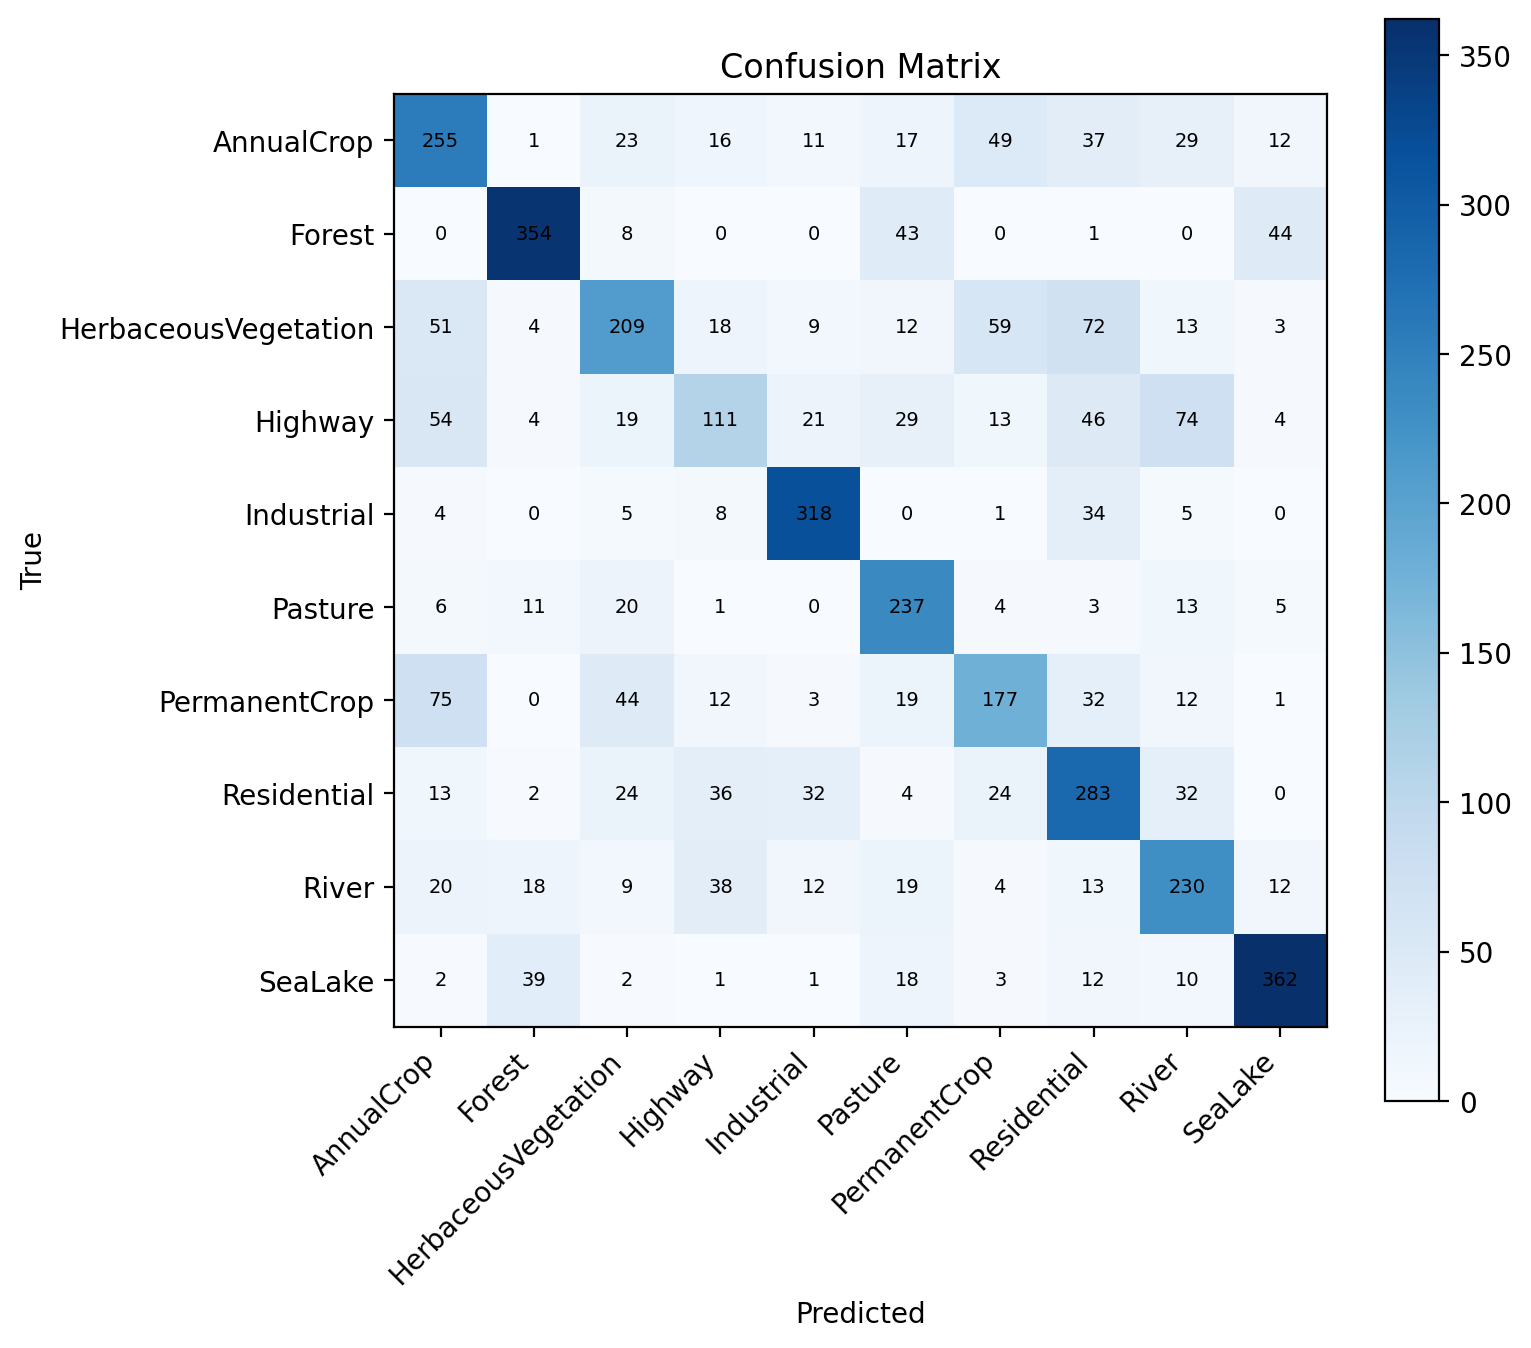
\includegraphics[width=0.85\textwidth]{confusion_matrix.png}
\caption{最终模型在测试集上的混淆矩阵}
\label{fig:confusion_matrix}
\end{figure}

\section{权重可视化与空间模式观察}

图~\ref{fig:first_layer_weights} 展示了第一层部分神经元权重恢复为图像后的可视化结果。

从可视化结果看，这些权重并没有表现出像卷积核那样清晰、规则的局部结构，
而是更接近高频颜色块和细粒度噪声纹理的组合。这一现象与模型结构本身有关：
MLP 在输入前先将图像展平，丢失了卷积网络常见的局部平移不变性，因此第一层权重
更像是在拟合全局像素分布中的颜色对比和粗纹理统计，而不是提取稳定的局部几何模式。

尽管如此，仍可以观察到一些神经元对绿色、棕色、蓝色等通道响应较强，
这说明模型确实利用了地表覆盖类别之间的颜色差异，例如：

\begin{itemize}
    \item 绿色主导的区域有助于区分 \texttt{Forest}、\texttt{Pasture} 等植被类；
    \item 蓝色成分更明显的权重有助于识别 \texttt{SeaLake}、\texttt{River}；
    \item 棕色与灰色条带可能对应农田、道路或工业地表的纹理信息。
\end{itemize}

整体而言，第一层权重中能看到一定颜色倾向，但空间模式并不稳定，这也是 MLP 相比 CNN
在图像任务上表达能力较弱的一个直观体现。

\begin{figure}[htbp]
\centering

\includegraphics[width=0.82\textwidth]{first_layer_weights.png}
\caption{第一层隐藏层部分权重的可视化结果}
\label{fig:first_layer_weights}
\end{figure}

\section{错例分析}

图~\ref{fig:misclassified_examples} 给出了测试集中的部分错分样例。
从这些样例可以看出，若只保留 $32 \times 32$ 分辨率并使用 MLP 进行分类，
当多个类别同时具有相似的颜色分布、条带纹理或块状结构时，模型容易出现误判。

本实验中较典型的错分现象包括：

\begin{itemize}
    \item 多张 \texttt{AnnualCrop} 被误分为 \texttt{PermanentCrop}，说明农田类之间的条带纹理、地块边界和颜色分布非常接近；
    \item 部分 \texttt{AnnualCrop} 被分为 \texttt{HerbaceousVegetation} 或 \texttt{Pasture}，反映出不同植被覆盖地物在低分辨率下难以仅凭颜色区分；
    \item 个别样本被误分为 \texttt{Highway} 或 \texttt{Industrial}，表明线性结构、裸露地表以及块状边界在视觉上具有一定相似性。
\end{itemize}

结合混淆矩阵来看，\texttt{Highway} 与 \texttt{River}、\texttt{Residential} 混淆较多，
说明在遥感视角下，线状目标和带状分布目标之间存在相当强的外观相似性。
此外，\texttt{PermanentCrop} 与 \texttt{AnnualCrop}、\texttt{HerbaceousVegetation}
的混淆也说明，植被类地物在没有卷积特征提取的情况下，确实较难通过简单的全连接网络完全分开。

\begin{figure}[htbp]
\centering
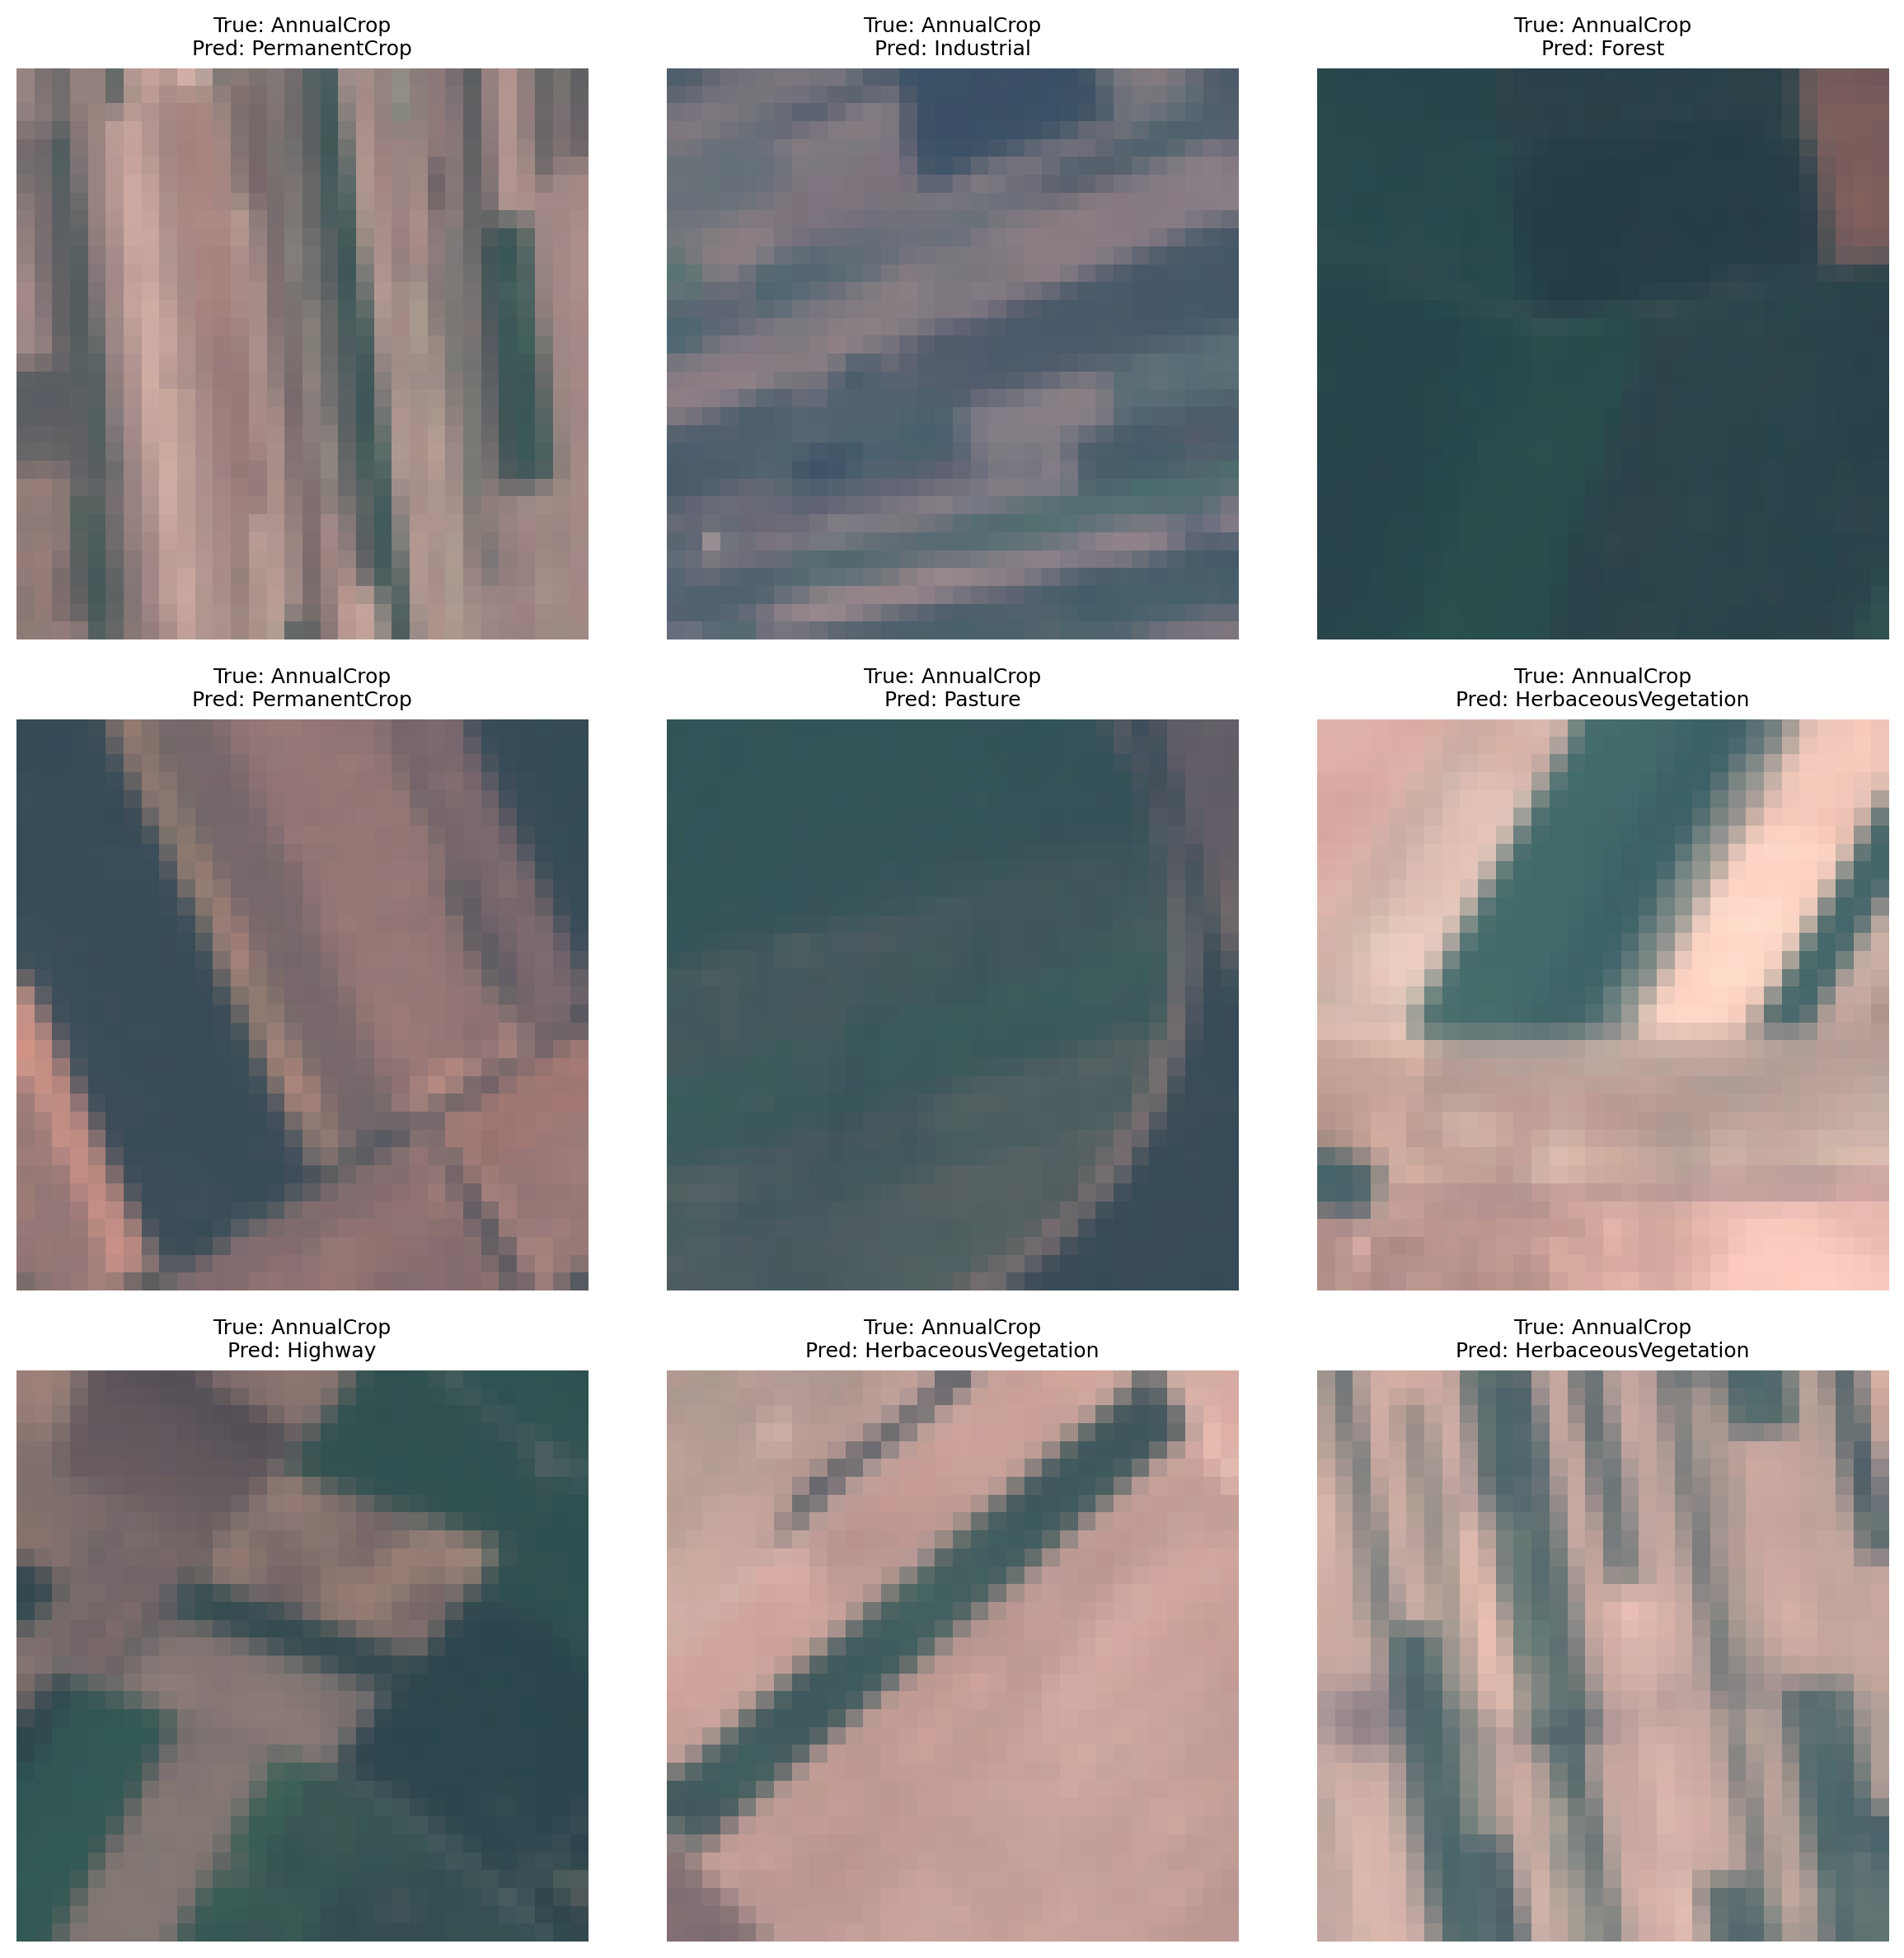
\includegraphics[width=0.82\textwidth]{misclassified_examples.png}
\caption{测试集中的部分错分样例}
\label{fig:misclassified_examples}
\end{figure}

\section{结论}

本实验完成了一个从零实现的三层 MLP 遥感图像分类系统，覆盖了自动微分、模型训练、
超参数搜索、最优权重保存、测试评估、混淆矩阵绘制、权重可视化和错例分析等全部环节。

从实验结果看：

\begin{itemize}
    \item 纯 MLP 在 EuroSAT 上能够达到 62.62\% 的测试准确率，说明其具备基本分类能力；
    \item 超参数搜索相比固定基线有稳定提升，说明模型性能对隐藏层宽度和正则化较敏感；
    \item 权重可视化与错例分析共同表明，MLP 更依赖颜色与粗纹理统计，而缺乏对局部空间结构的强建模能力。
\end{itemize}

如果继续改进，较自然的方向包括：加入更强的数据增强、重新设计学习率衰减策略、
尝试更大的隐藏层或更长训练、以及进一步使用更适合图像建模的卷积结构。
不过在本次作业限定的三层 MLP 框架下，当前结果已经较为合理地完成了任务要求。

\section*{提交信息}

以下两项内容需要在最终提交前替换为真实链接：

\begin{itemize}
    \item Public GitHub Repo：\RepoURL
    \item 模型权重下载地址：\WeightURL
\end{itemize}

\section*{复现实验命令}

以下命令可用于复现实验流程（根据实际目录位置调整）：

\begin{verbatim}
python -m src.search \
  --data_dir ./EuroSAT_RGB \
  --image_size 32 \
  --trials 8 \
  --epochs 20 \
  --run_name search_32

python -m src.test \
  --data_dir ./EuroSAT_RGB \
  --checkpoint ./outputs/search_32_best/checkpoints/best_model.npz \
  --run_name final_32_test
\end{verbatim}

\end{document}
